\documentclass[15pt]{beamer} % [12pt]
%\documentclass[15pt,aspectratio=1610]{beamer} % [12pt]
%\documentclass[15pt,letterpaper,handout]{beamer} % [12pt]

%\usepackage{fontspec}
\usepackage[spanish]{babel}
\usepackage[utf8]{inputenc}
\usepackage{textcomp}
\usepackage{multicol}

% For handout
%\usepackage{pgfpages}
%\pgfpagesuselayout{4 on 1}[letterpaper,landscape,border shrink=5mm]
% End of handout

\usetheme{Warsaw}
\expandafter\def\expandafter\insertshorttitle\expandafter{%
  \insertshorttitle\hfill%
  \insertframenumber\,/\,\inserttotalframenumber}

%\usetheme{PaloAlto}
%\usetheme{Marburg} % Barra azul a la derecha
%\usetheme{Madrid}

% What is this all about:
\title[Paralelización del filtro DNLM]{Implementación paralela de optimizaciones computacionales \\del
filtro DNLM para la plataforma Xeon Phi}
\subtitle{Trabajo Final de Graduaci\'on}
\institute[TEC]{Área Académica de Ingeniería en Computadores \\ Tecnológico de Costa Rica}
\date[Junio 2018]{11 Junio, 2018}
\author[M.\ Zumbado]{Ing.\ Manuel Zumbado Corrales}

%%%%%%%%%%%%%%%%%%%%%%%%%%%%%%%%%%%%%%%%%%%%%%%%%%%%%%%%%%%%%%%%%%%%%%%%%%%%
%  Notación

\usepackage{mathrsfs}                   % Calygraphic fonts for transforms

\renewcommand{\Re}{\operatorname{Re}}
\renewcommand{\Im}{\operatorname{Im}}

\newcommand{\prt}[1]{\ensuremath{\mathcal{#1}}}         %% partitioning
\newcommand{\img}[1]{\ensuremath{\mathcal{#1}}}         %% image as a set
\newcommand{\reg}[1][R]{\ensuremath{\mathcal{#1}}}      %% region
\newcommand{\pred}[1]{\ensuremath{\mathrm{#1}}}         %% predicate
\newcommand{\operat}[2]{\mathcal{#1}\left\{#2\right\}}
\newcommand{\transf}[1]{\mathscr{#1}}
\newcommand{\fourier}[1]{\transf{F}\left\{#1\right\}}
\newcommand{\ifourier}[1]{\transf{F}^{-1}\left\{#1\right\}}
\newcommand{\laplace}[1]{\transf{L}\left\{#1\right\}}
\newcommand{\ulaplace}[1]{\transf{L}_u\left\{#1\right\}}
\newcommand{\blaplace}[1]{\transf{L}_b\left\{#1\right\}}
\newcommand{\ilaplace}[1]{\transf{L}^{-1}\left\{#1\right\}}
\newcommand{\ztrans}[1]{\transf{Z}\left\{#1\right\}}
\newcommand{\iztrans}[1]{\transf{Z}^{-1}\left\{#1\right\}}
\newcommand{\zutrans}[1]{\transf{Z}_u\left\{#1\right\}}
\newcommand{\exceq}{\ensuremath{\overset{!}{=}}}

\newcommand{\signum}{\operatorname{signum}}
\newcommand{\pos}{\operatorname{pos}}
\newcommand{\val}{\operatorname{val}}
\newcommand{\vct}[1]{\ensuremath{\underline{\mathbf{#1}}}}
\newcommand{\pix}[1]{\ensuremath{\mathbf{#1}}}
\newcommand{\mat}[1]{\ensuremath{\mathbf{#1}}}
\newcommand{\vctmu}{\vct{\boldsymbol{\mu}}}
\newcommand{\vctzeta}{\vct{\boldsymbol{\zeta}}}
\newcommand{\vctpi}{\vct{\boldsymbol{\pi}}}
\newcommand{\vctvarphi}{\vct{\boldsymbol{\varphi}}}
\newcommand{\raum}[1]{\ensuremath{\mathbb{#1}}}
\newcommand{\matSigma}{\mat{\boldsymbol{\Sigma}}}
\newcommand{\matLambda}{\mat{\boldsymbol{\Lambda}}}
\newcommand{\matPsi}{\mat{\boldsymbol{\Psi}}}
\newcommand{\matPhi}{\mat{\boldsymbol{\Phi}}}
\newcommand{\row}[2]{\ensuremath{\mathbf{\underline{#1}_{#2(\cdot)}}}}
\newcommand{\col}[2]{\ensuremath{\mathbf{\underline{#1}_{(\cdot) #2}}}}
\newcommand{\seq}[1]{\ensuremath{#1}}
\newcommand{\set}[1]{\ensuremath{\mathcal{#1}}}
\newcommand{\gset}[1]{\ensuremath{#1}} %% set for greek symbols
\newcommand{\front}[1]{\widehat{\set{#1}}}
\newcommand{\setlambda}{\set{\boldsymbol{\lambda}}}
\newcommand{\klass}[1]{\ensuremath{\mathpss{#1}}}
\newcommand{\graph}[1]{\ensuremath{\mathsf{#1}}}
\newcommand{\lab}[1]{\ensuremath{\mathpss{L}(#1)}}
\newcommand{\myfrac}[2]{{\footnotesize #1/#2}}
\newcommand{\ifthenspc}{\rule{3mm}{0mm}}
\newcommand{\point}[1]{\ensuremath{\mathsf{#1}}}
\newcommand{\estim}[1]{\ensuremath{\hat{#1}}}
\newcommand{\numset}[1]{\ensuremath{\mathbb{#1}}}
\newcommand{\tuple}[1]{\ensuremath{\left\langle#1\right\rangle}}
\newcommand{\conj}[1]{\ensuremath{{{#1}^{\ast}}}}
\newcommand{\base}[1]{\set{#1}}
\newcommand{\zeron}[1]{\ensuremath{\underset{\uparrow}{#1}}}
\newcommand{\sysT}{\ensuremath{\mathcal{T}}}
\newcommand{\sys}[1]{\ensuremath{\sysT\left[#1\right]}}
\newcommand{\sen}{\operatorname{sen}} % sinus in spanish (seno)
\newcommand{\senh}{\operatorname{senh}} % sinus hiperbolicus in spanish (seno)
\newcommand{\arcsen}{\operatorname{arcsen}} % arcus sinus hiperbolicus in spanish (arcoseno)
\newcommand{\sgn}{\operatorname{sgn}} % signus
\newcommand{\roc}{\text{ROC: }}

\newcommand{\code}[1]{\texttt{#1}}
\newcommand{\conv}{\ensuremath{\ast}}
\newcommand{\cconv}{\ensuremath{\;\,\text{\footnotesize{N}}\!\!\!\!\!\!\bigcirc}}
\newcommand{\Ln}{\operatorname{Ln}}
\newcommand{\sa}{\operatorname{sa}}
\newcommand{\senc}{\operatorname{senc}}
\newcommand{\si}{\operatorname{si}}

%% Natural, Integer and Real Numbers
\newcommand{\setA}{\ensuremath{\mathbb{A}}}
\newcommand{\setB}{\ensuremath{\mathrm{I\negthinspace B}}}
\newcommand{\setC}{\ensuremath{\mathbb{C}}}
\newcommand{\setD}{\ensuremath{\mathrm{I\negthinspace D}}}
\newcommand{\setE}{\ensuremath{\mathrm{I\negthinspace E}}}
\newcommand{\setF}{\ensuremath{\mathrm{I\negthinspace F}}}
\newcommand{\setG}{\ensuremath{\mathbb{G}}}
\newcommand{\setH}{\ensuremath{\mathrm{I\negthinspace H}}}
\newcommand{\setI}{\ensuremath{\mathbb{I}}}
\newcommand{\setJ}{\ensuremath{\mathbb{J}}}
\newcommand{\setK}{\ensuremath{\mathrm{I\negthinspace K}}}
\newcommand{\setL}{\ensuremath{\mathrm{I\negthinspace L}}}
\newcommand{\setM}{\ensuremath{\mathrm{I\negthinspace M}}}
\newcommand{\setN}{\ensuremath{\mathrm{I\negthinspace N}}}
\newcommand{\setO}{\ensuremath{\mathbb{O}}}
\newcommand{\setP}{\ensuremath{\mathrm{I\negthinspace P}}}
\newcommand{\setQ}{\ensuremath{\mathbb{Q}}}
\newcommand{\setR}{\ensuremath{\mathrm{I\negthinspace R}}}
\newcommand{\setS}{\ensuremath{\mathbb{S}}}
\newcommand{\setT}{\ensuremath{\mathbb{T}}}
\newcommand{\setU}{\ensuremath{\mathbb{U}}}
\newcommand{\setV}{\ensuremath{\mathbb{V}}}
\newcommand{\setW}{\ensuremath{\mathbb{W}}}
\newcommand{\setX}{\ensuremath{\mathbb{X}}}
\newcommand{\setY}{\ensuremath{\mathbb{Y}}}
\newcommand{\setZ}{\ensuremath{\mathbb{Z}}}


%%%%%%%%%%%%%%%%%%%%%%%%%%%%%%%%%%%%%%%%%%%%%%%%%%%%%%%%%%%%%%%%%%%%%%%%%%%%

\begin{document}
\graphicspath{{./}{./fig/}}

\begin{frame}
  \titlepage
\end{frame}


\begin{frame}{Contenido}
  \tableofcontents
\end{frame}

% Título para el contexto
\section{Preprocesamiento de imágenes}

\begin{frame}{Contexto}

\begin{columns}
    \column{.45\textwidth}
    \begin{enumerate}
    \item <1-| alert@1> Imagen de entrada
    \item <2-| alert@2> Imagen filtrada
    \item <3-| alert@3> Segmentaci\'on
    \end{enumerate}
    \column{.5\textwidth}
    \only<1>{
\includegraphics[width=0.9\textwidth]{cisplatino_original}}
    \only<2>{
\includegraphics[width=0.9\textwidth]{cisplatino_preprocessed}}
    \only<3>{
\includegraphics[width=0.9\textwidth]{cisplatino_segmentation}}
  \end{columns}
\end{frame}

\begin{frame}{Problema}
  
  \begin{itemize}
  \item Dependiendo del tema, combine con folio anterior
  \item Explique problema concreto a resolver
  \end{itemize}
\end{frame}

\begin{frame}{Objetivos}
  
  \begin{itemize}
  \item Palabras clave de objetivo general
  \item Objetivos específicos resumidos 
  \end{itemize}
\end{frame}


\section{Solución}

\subsection{Segmentación de nematodos}


\begin{frame}{Segmentación en dos niveles}{{\tiny{Olman Gómez, 2009}}}
  % Coloque el diagrama de bloques detallado de su solución
  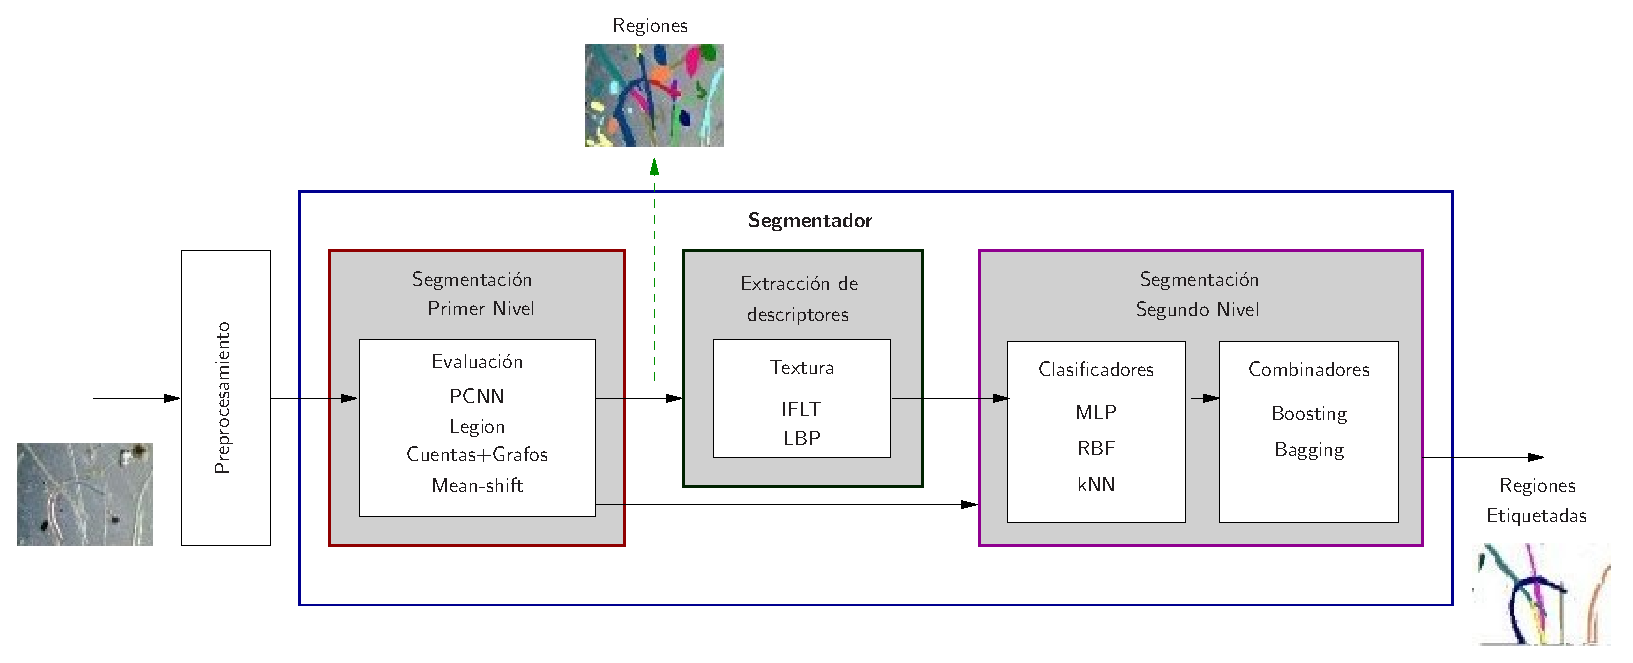
\includegraphics[width=\textwidth]{gomezsegm_fixed}
\end{frame}

\begin{frame}{Bloques}
  % Aproveche el medio visual para dejar clara LA IDEA (no hay tiempo
  % para detalle teórico).
  \begin{columns}
    \column{.45\textwidth}
    \begin{enumerate}
    \item <1-| alert@1> Entrada
    \item <2-| alert@2> Filtro Mediana
    \item <3-| alert@3> Contraste
    \item <4-| alert@4> Gradiente
    \item <5-| alert@5> Estimación Umbral
    \item <6-| alert@6> Cuencas
    \item <7-| alert@6> Combinación
    \end{enumerate}
    \column{.5\textwidth}
    \only<1>{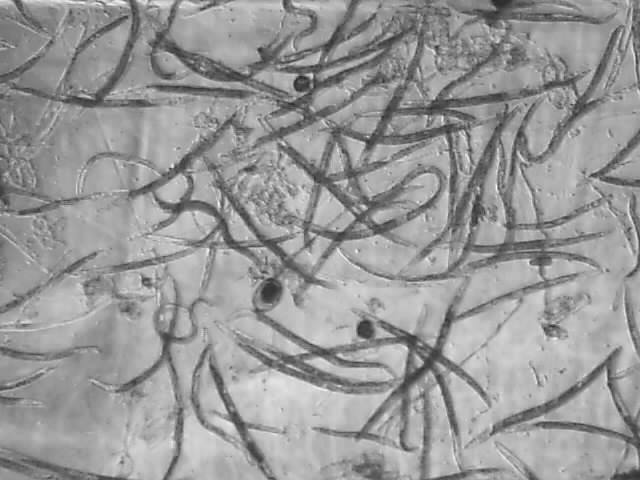
\includegraphics[width=0.9\textwidth]{nematodos}}
    \only<2>{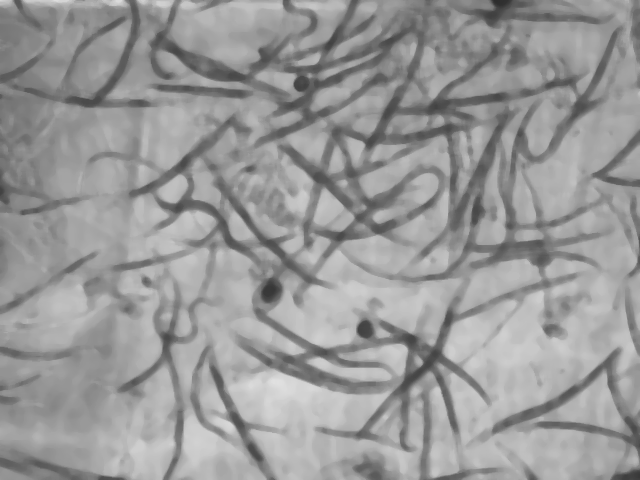
\includegraphics[width=0.9\textwidth]{cwagm1}}
    \only<3>{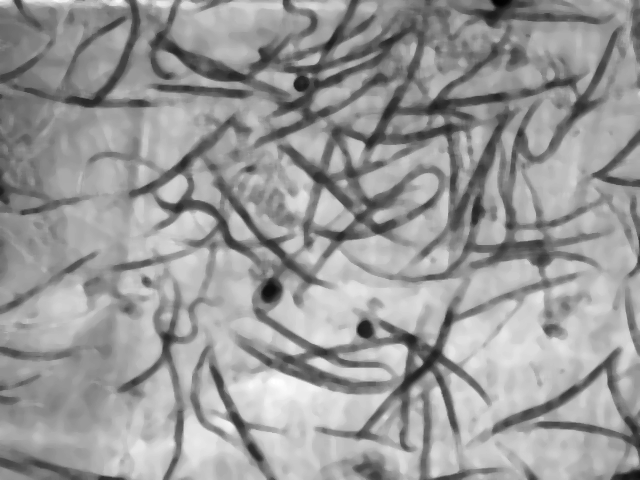
\includegraphics[width=0.9\textwidth]{cwagm2}}
    \only<4>{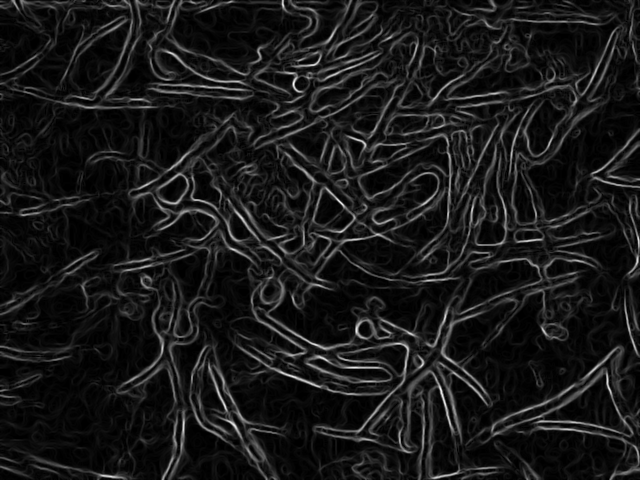
\includegraphics[width=0.9\textwidth]{cwagm3}}
    \only<5>{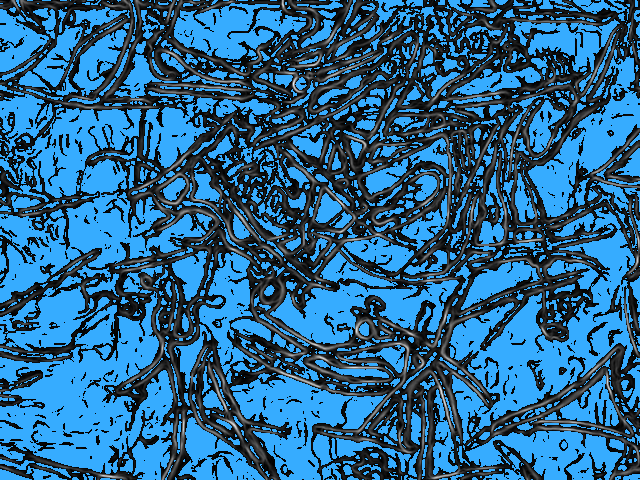
\includegraphics[width=0.9\textwidth]{cwagm2b}}
    \only<6>{
\includegraphics[width=0.9\textwidth]{cwagm4}}
    \only<7>{
\includegraphics[width=0.9\textwidth]{cwagm5}}
  \end{columns}
\end{frame}

\section{Resultados}

\begin{frame}{Algoritmo de segundo nivel}
  
  \begin{enumerate}
  \item Características de Textura (IFLT, LBP)
  \item Clasificadores neuronales (MLP, RBF), estadísticos (kNN)
  \item Mezcla de clasificadores (AdaBoosting)
  \end{enumerate}

  % PPV: valor predictivo positivo
  %
  % La matriz de confusión cruda corresponderá a la acumulación en cada ite-
  % ración de la clasificación de las regiones de la imagen de validación,
  % usando el clasificador entrenado con el resto de las imágenes.
  %
  % La matriz de sensibilidad da la probabilidad de que un objeto de
  % determinada clase sea correctamente asignado.
  % Se obtiene dividiendo los elementos de C cruda entre
  % el número de objetos en la correspondiente clase verdadera.
  %
  % La matriz de valor predictivo positivo (PPV) da la probabilidad que un
  % objeto asignado a una clase en realidad pertenezca a esa clase.
  % Se obtiene dividiendo los elementos de cada fila entre el número total
  % de objetos asignados a esa clase.

  \begin{center}
    {\footnotesize Matrices de confusión para la combinación con}

    {\footnotesize AdaBoost de MLP para la unión de descriptores con 
      vecindario de 8 y 16}
    \begin{tabular}{|c|cc|cc|cc|}
      \hline
      & \multicolumn{2}{c|}{Cruda} & \multicolumn{2}{c|}{Sensibilidad} & 
      \multicolumn{2}{c|}{VPP} \\
      \hline
      Asignada$\backslash$Real& Fondo & Nem.& Fondo & Nem.& Fondo & Nem. \\
      \hline
      Fondo & 456 & 51 & 0,877 & 0,236 & 0,899 & 0,101 \\
      Nematodo & 64 & 165 & 0,123 & 0,764 & 0,279 & 0,721 \\
      \hline
      & \multicolumn{6}{c|}{Precisión = 0,844}\\
      \hline
    \end{tabular}
  \end{center}
\end{frame}


\begin{frame}{Conclusiones}
  
  \begin{itemize}
  \item Resuma las conclusiones y recomendaciones
  \item No use texto completo sino únicamente palabras clave
  \end{itemize}
  
\end{frame}

\begin{frame}{Trabajo futuro}
  
  \begin{itemize}
  \item Resuma ideas para trabajos futuros
  \end{itemize}
  
\end{frame}


\section{Resumen}

\begin{frame}{Resumen}
  \tableofcontents
\end{frame}

\end{document}
